\chapter{Algorithms and Approaches for Terrain LOD}
\section{Basics of Terrain LOD}
\subsection{Terrain Data Representation}
\subsubsection{Heightmaps}
One way of representing terrains is using \textit{heightmaps}.
A heightmap is a $n\times n$-grid that contains 
the height value $y$ for each $(x,z)$-position\footnote{We always denote $y$ for the up direction except if explicitly stated otherwise.}.
Positions are always spaced evenly in a grid-like manner,
but the distance between any two neighboring positions is variable.

The main advantage of heightmaps is that they allow for very simple storage and manipulation of height data, e.g. in form of images,
where low color values represent low areas of terrain and vice versa for
high color values. For a grayscale image, up to 256 height values can be used and for an RGB image,
more than 16 million height values are supported.
Looking up a height value for a given $(x,z)$-position is easy as well,
which consists of a simple lookup at the given position in the image.
Figure~\ref{fig:dom} shows a $2000 \times 2000$ heightmap of the mountain Dom in Valais, Switzerland.
\begin{figure}
  \centering
  
\includegraphics[width=0.44\textwidth]{dom}
  \caption{$2000 \times 2000$ heightmap of the mountain Dom in Valais, Switzerland retrieved from SwissTopo \cite{alti3d}.}\label{fig:dom}
\end{figure}

\subsubsection{Triangulated Irregular Networks}
An alternative to the heightmap is the \textit{triangulated irregular network (TIN)} data structure.
A TIN consists of a collection of 3D vertices, where 
the arrangement of vertices can be irregular. Figure~\ref{fig:tin-example} shows 
an example of a TIN.
\begin{figure}
  \centering
  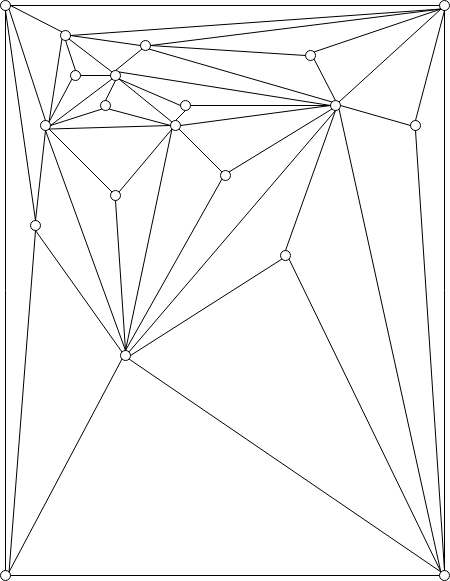
\includegraphics[width=0.52\textwidth]{tin-example}
  \caption{Example of a TIN. Note that the upper area represents a terrain area with many changes 
  (e.g. mountains, hills, etc.), and the lower area represents an area with few changes (e.g. flat areas).}\label{fig:tin-example}
\end{figure}

The main advantage of TINs is that fewer polygons need to be used for 
e.g. smooth terrain areas. Another advantage is that
special terrain features can be modelled 
which are usually difficult to model with heightmaps, such as overhangs, cliffs and caves, 
The disadvantage of TINs, however, is that the full $(x,y,z)$ coordinates need to be stored,
whereas with heightmaps, only the height value $y$ needs to be stored.

\subsection{Bintrees and Quadtrees}
\textit{Binary triangle trees (bintrees)} and \textit{quadtrees} are 
recursive data structures based on triangles and quads respectively.
A bintree consists of up to two child triangles, both of which in turn also consist of up to two child triangles each, and so on,
as shown in figure~\ref{fig:bintree-example}.

\begin{figure}
  \centering
  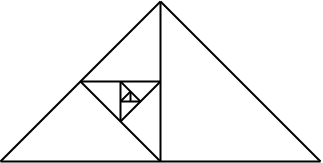
\includegraphics[width=0.43\textwidth]{bintree-example}
  \caption{Example of a bintree.}\label{fig:bintree-example}
\end{figure}

Quadtrees are structured similarly, with a quad consisting of up to four child quads, and each child quad consisting
of up to four child quads, and so on.
Figure~\ref{fig:quadtree-example} shows an example of a quadtree.

\begin{figure}
  \centering
  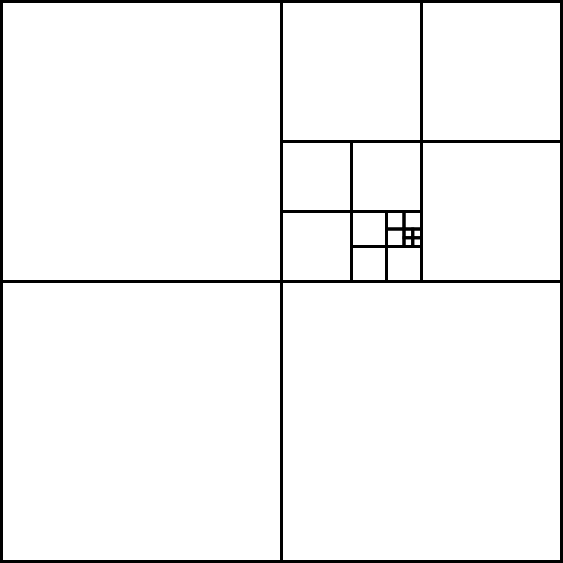
\includegraphics[width=0.52\textwidth]{quadtree-example}
  \caption{Example of a quadtree.}\label{fig:quadtree-example}
\end{figure}

The main advantage of bintrees and quadtrees is that 
LOD can be modelled very naturally with them.
Bintree/quadtree sections with few children correspond to a low LOD and 
vice versa for bintree/quadtree sections with many children.

\subsection{Potential Problems During Terrain Rendering}
While terrain LOD algorithms dramatically improve the performance of terrain rendering, 
there are certain faults that can occur during rendering. 

\paragraph{Cracks} Cracks and holes in terrains can appear when a higher LOD terrain section is bordered 
by a lower LOD terrain section. The main problem is that when a vertex $v_{\text{high}}$ of a higher LOD terrain section lies on the edge $e_{\text{low}}$
of a lower LOD terrain section and the $y$ coordinate of $v_{\text{high}}$ is greater or less than the 
height of $e_{\text{low}}$ at that point, the difference in height causes the crack to appear, as shown in figure~\ref{fig:crack-example}.
Cracks can be solved by either 
\begin{itemize}
  \item removing the vertex in question (in figure~\ref{fig:crack-example} vertex $v_{\text{high}}$),
  \item inserting more vertices so that the LOD,
  \item or by force splitting the mesh so that the LOD does not contain such vertices that can cause holes.
\end{itemize}

\begin{figure}
  \centering
  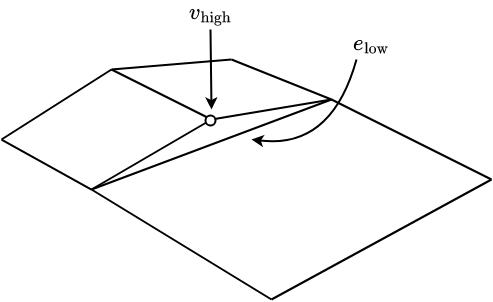
\includegraphics[width=0.6\textwidth]{crack-example}
  \caption{Example of a crack.}\label{fig:crack-example}
\end{figure}

\paragraph{Popping} The phenomenon of \textit{popping} occurs when the camera is moving 
and the transition of the terrain's LOD level causes visual pops to appear.
Popping decreases the realism of the terrain and should be as minimal as possible.
Popping can be reduced by introducing \textit{vertex morphing}, 
i.e. by animating the transition of one LOD level to the next seamlessly.

\section{ROAM}
ROAM (short for \textbf{R}eal-time \textbf{O}ptimally \textbf{A}dapting \textbf{M}eshes) 
is a terrain LOD algorithm developed by Duchaineau \textit{et al.} \cite{roam} published in 1997.
ROAM represents the terrain mesh using bintrees. The algorithm is mainly CPU-based, which 
can be attributed to the less developed state of GPU programming at the time.

\subsection{General Idea}
The central idea of the algorithm is to use temporal coherence: the mesh from a previous frame $\mathbf{T}_{f-1}$ is used to compute 
the mesh of the current frame $\mathbf{T}$, rather than building up the mesh from ground up for each frame.
This is done using two priority queues: a split queue $\mathcal{Q}_s$ and a merge queue $\mathcal{Q}_m$.
The split queue contains splittable triangle pairs $()$
and the merge queue contains mergable triangle pairs $(T,T_B)$.
The elements of the priority queues are ordered by 
various geometric error metrics, which will be explained in the subsection ``Error Metrics''.
ROAM is a greedy algorithm, meaning it will always compute the most optimal mesh for each frame.

% [The algorithm is described in pseudocode below in algorithm 1.

% \newcommand{\pushcode}[1][1]{\hskip\dimexpr#1\algorithmicindent\relax}
% \begin{algorithm}
%   \caption{ROAM incremental greedy update}\label{alg:cap}
%   \begin{algorithmic}[1]
%   \Procedure{RoamIncrementalUpdate}{}
%   \If{$f = 0$} \Comment{Initial frame}
%     \State $\mathbf{T} \gets \text{base triangulation}$.
%     \State Clear $\mathcal{Q}_s, \mathcal{Q}_m$.
%     \State Compute priorities for triangles and diamonds $\in \mathbf{T}$ 
%     \State and insert them into $\mathcal{Q}_s$ and $\mathcal{Q}_m$.
%   \Else
%     \State $\mathbf{T} \gets \mathbf{T}_{f-1}$.
%     \State Update priorities for all elements $\in \mathcal{Q}_s$, $\mathcal{Q}_m$.
%   \EndIf
%   \While{\textbf{not} $\mathbf{T}$ is target size/accuracy \textbf{or} \\
%   \hskip\algorithmicindent maximum split priority $>$ minimum merge priority}
%     \If{$\mathbf{T}$ is too large or accurate}
%       \State Find lowest priority $(T, T_B) \in \mathcal{Q}_m$. 
%       \State Merge $(T, T_B)$.
%       \State Remove all merged children from $\mathcal{Q}_s$.
%       \State Add merge parents $T, T_B$ to $\mathcal{Q}_s$.
%       \State Add all newly mergable diamonds to $\mathcal{Q}_m$.
%     \Else \Comment{$\mathbf{T}$ is too small or inaccurate}
%       \State Find highest priority $T \in \mathcal{Q}_s$.
%       \State Force-split $T$.
%       \State Remove $T$ and other split triangles from $\mathcal{Q}_s$.
%       \State Add any new triangles $\in \mathbf{T}$ to $Q_s$.
%       \State Remove from $Q_m$ any diamonds whose children were split.
%       \State Add all newly mergable diamonds to $\mathcal{Q}_m$.
%     \EndIf
%   \EndWhile
%  \EndProcedure
%   \end{algorithmic}
% \end{algorithm}]

\subsection{Error Metrics}
The error metrics used for the priority queues are the following:

\paragraph{Wedgies} The so-called \textit{Wedgies} are nested bounding volumes around triangles that are computed 
while building an initial mesh at the beginning of the algorithm.
A wedgie is defined to contain the entire $x$ and $z$ extent\footnote{The original ROAM paper uses $z$ for the up direction. For the sake of consistency with the rest of this report, we will use $y$ as the up direction here.}
of a triangle and the height $y$ including some additional space above and below the highest and lowest points,
respectively.

\paragraph{Geometric Screen Distortion}

\paragraph{Other Metrics} Other priority metrics mentioned include 

\subsection{Reported Performance and Conclusion}
Duchaineau et al. report that the runtime of ROAM is proportionate to the 
number of triangle changes.

%\section{Röttger's Quadtree-based Algorithm}
%TODO

\section{GeoMipMapping}
\textit{Geometrical Mipmapping (GeoMipMapping)} is a terrain LOD approach developed by de Boer \cite{geomipmapping} in the year 2000.

\subsection{General Idea}
The central idea of GeoMipMapping is its analogy to texture mipmapping: just like how textures of far away objects are rendered using lower resolution texture mipmaps,
terrain areas that are far away from the camera should also be rendered with a lower resolution mesh.
This is achieved by splitting up the terrain into so-called \textit{blocks} (also called \textit{patches}) of a fixed width $2^n + 1$ for an arbitrary $n$.
At each LOD level, the number of vertices on one side of a block is $2^{l}+1$, where $0\leq l \leq n$ is the current LOD level\footnote{The original paper uses 0 to denote the maximum LOD level and vice-versa for the minimum LOD level. }.
For example, a $5 \times 5$ terrain block contains $2^2 + 1 = 5$ vertices on one side at the maximum LOD level 2, $2^1 + 1 = 3$ vertices at LOD level 1 and $2^0 + 1 = 2$ vertices at the minimum LOD level 0, as
shown in figure~\ref{fig:geomipmapping-patch-example}.


\begin{figure}
  \centering
  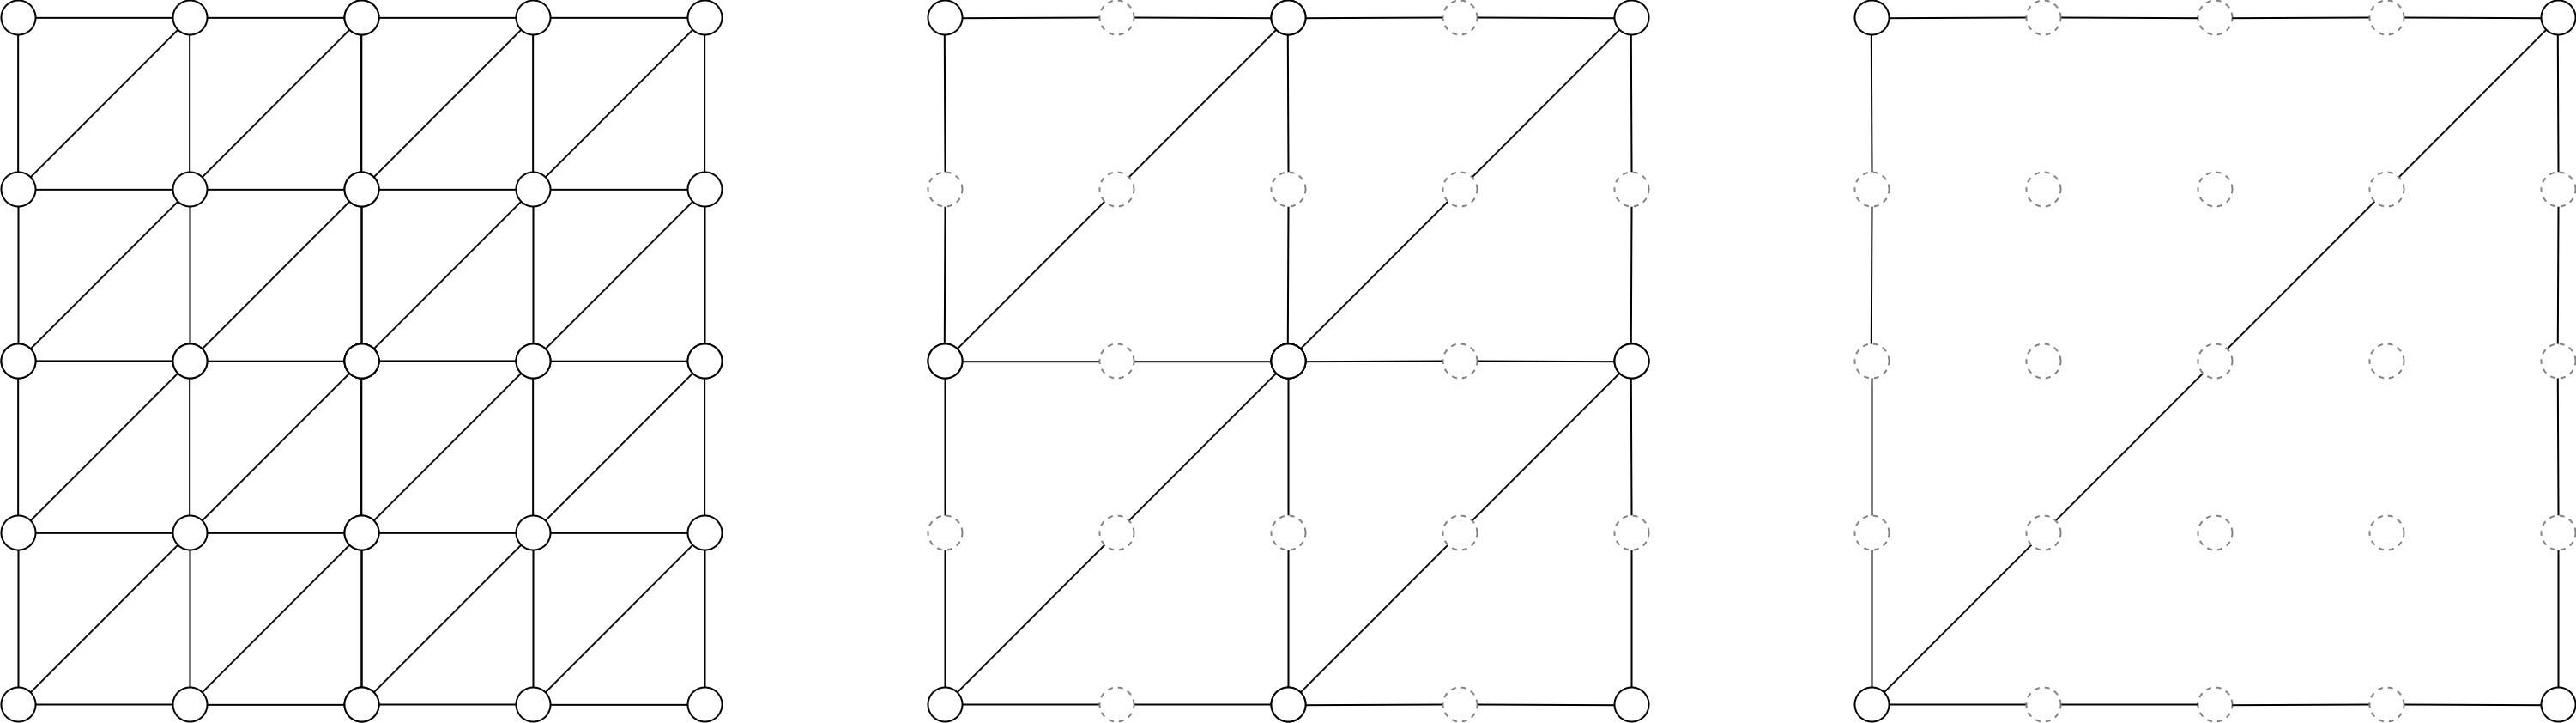
\includegraphics[width=1\textwidth]{geomipmapping-patch-example}
  \caption{Example of a $5 \times 5$ block with the maximum LOD level of 2 (left), LOD level of 1 (middle) and minimum LOD level of 0 (right). The omitted vertices of the lower LOD blocks are shown here as dotted circles.}\label{fig:geomipmapping-patch-example}
\end{figure}

%\section{Geometry Clipmaps}
%TODO

%\section{CDLOD}
%TODO

